\section{One factor at a time proves nothing here}
\label{sec:ofat}

We swept six parameters one at a time --- total precision (4--12), window
size (2--8), overlap (0--3), candidate count (1--16), beam width (1--4096),
and shots (16--16384) --- holding the rest at their defaults, across three
small $(N,a)$ pairs, 15 trials per parameter value.

\textbf{Every one of the 435 trials succeeded.} Table~\ref{tab:ofat}
reports the sweep; every cell is $15/15$, with a $95\%$ Wilson lower bound of
$0.796$. A factorial logistic regression of success on the three noise
levels (Fig.~\ref{fig:logistic}) likewise finds nothing: the largest
coefficient is two-qubit depolarising error at $-0.452$, and all three
confidence intervals cross zero.

This is a genuine null result with a specific cause rather than an absence of
evidence. At the orders reachable here the continued-fraction search absorbs
substantial phase error, so a configuration that is theoretically
under-resolved still recovers the right order. \textbf{The methodological
consequence is the point:} a one-factor-at-a-time design applied to this
pipeline will report that it has no failure modes, and be wrong. We report
the null in full because it is what motivated the design of
Sec.~\ref{sec:combined}, and because anyone characterising a comparable
pipeline is likely to start the same way.

\begin{table}[htbp]
\centering\small
\caption{Single-parameter sweep. Each row is one parameter value at 15
seed-paired trials with all other parameters at their defaults. Every cell
succeeded; the interval is a $95\%$ Wilson score interval, whose lower bound
of $0.796$ is what 15 successes out of 15 supports. From
\texttt{phase1\_ofat.csv}.}
\label{tab:ofat}
\begin{tabular}{@{}llrl@{}}
\toprule
Parameter & Values swept & Trials & Success \\
\midrule
Total precision $\ell$   & 4, 6, 8, 10, 12          & 75 & 15/15 each \\
Window size $\ell_w$     & 2, 3, 4, 6               & 60 & 15/15 each \\
Overlap $o$              & 0, 1, 2, 3               & 60 & 15/15 each \\
Candidate count $k$      & 1, 2, 4, 8, 16           & 75 & 15/15 each \\
Beam width $P$           & 1, 4, 16, 64, 256        & 75 & 15/15 each \\
Shots $S_w$              & 16, 64, 256, 1024, 4096, 16384 & 90 & 15/15 each \\
\midrule
\textbf{Total}           &                          & \textbf{435} & \textbf{435/435} \\
\bottomrule
\end{tabular}
\end{table}

\begin{figure}[htbp]
\centering
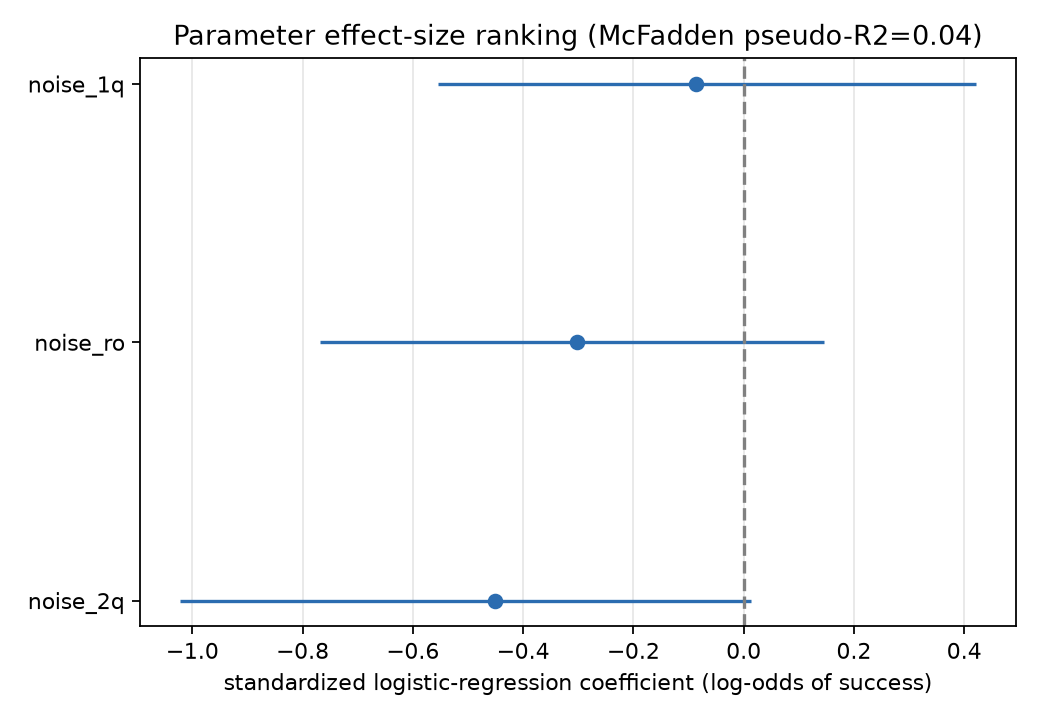
\includegraphics[width=0.78\linewidth]{../Data/failure_study/plots/logistic_effect_sizes.png}
\caption{\textbf{Standardised logistic-regression effect sizes for the three
noise channels.} Two-qubit depolarising error is the largest single driver
at $-0.452$, but all three intervals cross zero: at single-source levels, no
noise channel is individually distinguishable from none. The interaction
that does matter is in Sec.~\ref{sec:noise}. Rendered from
\texttt{phase1\_ofat.csv}.}
\label{fig:logistic}
\end{figure}
